\documentclass[11pt]{article}
\setlength{\parskip}{.08in} 
\renewcommand\arraystretch{1.2}
\usepackage{commath}
\usepackage{listings}
\usepackage{hyperref} 
\usepackage{float}
\setlength{\parindent}{0in}

\lstdefinestyle{mystyle}{
basicstyle=\fontsize{10}{7}\selectfont\ttfamily
}
\lstset{style=mystyle}

% Added packages
\usepackage{setspace}
\usepackage{enumerate}
\usepackage{bm}
\usepackage{amsmath}
\makeatletter
\renewcommand*\env@matrix[1][\arraystretch]{%
  \edef\arraystretch{#1}%
  \hskip -\arraycolsep
  \let\@ifnextchar\new@ifnextchar
  \array{*\c@MaxMatrixCols c}}
\makeatother
%\usepackage[dvips, bookmarks, colorlinks=true, plainpages = false, 
%citecolor = green, urlcolor = blue, filecolor = blue] {hyperref}
%\usepackage[font=small,format=plain,labelfont=bf,up,textfont=it,up]{caption}

% Set the beginning of a LaTeX document
\usepackage{graphicx}
\graphicspath{ {./images/} }

%\usepackage{endnotes}
%\let\footnote=\endnote

\usepackage{titlesec}
\titleformat{\section}
  {\normalfont\fontfamily{phv}\fontsize{14}{17}\selectfont}{\thesection}{1em}{}

\oddsidemargin 0.25in
\evensidemargin 0.25in 

\headheight 0.0in
\headsep 0.0in
\topmargin -0.25in

\textwidth 6.0in 
\textheight 9.0in 

\paperheight 11.0in
\paperwidth 8.5in

\begin{document}

\title{Extrapolation of Climate Data using Numerical Methods}
\author{Philippe Nadon\footnote{Corresponding author: nadon@ualberta.ca}}

\date{ \today}
\maketitle

{\small Faculty of Science, University of Alberta}\\
{\small Camrose, Alberta, Canada}\\[0.5cm]

\thispagestyle{empty}

%\onehalfspacing
\doublespacing

\begin{abstract}
Climate change is currently a major concern for society, due to the irreversible damage predicted by our models if we continue our current trend of excessive emissions and pollution. In this paper various methods of data-fitting and extrapolation are explored, and compared to see how accurately they represent the data provided.

\end{abstract}

\textbf{Keywords:} Climate, Numerical Methods, Extrapolation

\newpage

\setcounter{page}{1}

\section{Introduction}
Data is obtained from Berkeley Earth, the table representing the "Global Average Temperature Anomaly with Sea Ice Temperature Inferred from Air Temperatures". This data spans from 1850 to 2018, and shows us how global temperatures have changed in the last 168. Using this data, we can use the method of least squares to fit various equations onto this data, and then extrapolate the data's trend into the future. These include a linear, quadratic, and cubic fit, which are approximated by solving an $nxn$ matrix, where n is the degree of the polynomial + 1. Afterwards, two more fits are used, an exponential fit and finally 2 different combinations of a polynomial and exponential. These last three are solved using Matlab's \textit{lsqcurvefit} function. Although modern techniques are far more sophisticated, these results will still give us a general understanding of what will happen if we do not change our habits which impact the planet's climate.

\section{Methods}
Multiple equations were used to fit the data so we could compare their respective accuracies and predictions. They are listed below:
\begin{equation}\label{eq:linear}
linear = \alpha + \beta x
\end{equation}
\begin{equation}\label{eq:quadratic}
quadratic = \alpha + \beta x + \gamma x^2
\end{equation}
\begin{equation}\label{eq:cubic}
cubic = \alpha + \beta x + \gamma x^2 + \delta x^3
\end{equation}
\begin{equation}\label{eq:exp}
exponential = \alpha + e^{\beta x}
\end{equation}
\begin{equation}\label{eq:mix1}
mixed_1 = \alpha + (\gamma + \delta x)e^{\beta x}
\end{equation}
\begin{equation}\label{eq:mix2}
mixed_2 = \alpha + (\gamma + \delta x + \epsilon x^2)e^{\beta x}
\end{equation}

\subsection{ Linear, Quadratic, Cubic Fits}
The following code was used to calculate the best fit for the data, using equations \eqref{eq:linear}, \eqref{eq:quadratic}, and \eqref{eq:cubic}. The method of least squares can be solved by forming the problem into a system of linear equations in the form $Ax = B$, and solving for x.

\begin{lstlisting}[language=Matlab, style=myStyle]
function res = extrapolatePolyToYear( t, data, degree)
    N = length(data);
    rows = degree + 1;
    A = zeros( rows, rows);
    B = zeros( rows, 1);
    
    for n = 1:N
        for i = 1:rows
            % for A:
            % The diagonal entries:
            A(i, i) = A(i, i) + t(n) ^ (2 * ( i - 1));
            % The upper / lower entries (mirror along diagonal)
            for j = 1:(i - 1)
                A( i, j) = A(i, j) + t(n) ^ ( i + j - 2);
                A( j, i) = A(i, j);
            end
            
            % for B:
            B(i) = B(i) + data(n) * t(n) ^ (i - 1);
        end
    end
    disp(A);
    disp(B);

    res = linsolve( A, B);
end
\end{lstlisting}
This function receives an array containing t values, an array of data, and the degree of polynomial you wish to fit onto the data. It then returns an array containing the coefficients of the polynomial that is to be fit onto the data.\\

\subsection{ Exponential and Mixed Fits}
Equations \eqref{eq:exp}, \eqref{eq:mix1}, and \eqref{eq:mix2} were simpler to solve, but involved modifying the initial guesses until the plot fit well. The plot was done using the Matlab function \textit{lsqcurve}. The initial guesses are as follows:\\
Exponential:
\[ \alpha = -0.4, \beta = 0.02, \gamma = 0.1 \]
Exponential and Linear:
\[ \alpha = -0.5, \beta = 0.02, \gamma = -0.4, \delta = -0.002 \]
Exponential and Quadratic:
\[ \alpha = -0.5, \beta = 0.02, \gamma = -0.4, \delta = -0.002, \epsilon = 0.03 \]

\section{Results}
\subsection{ Linear, Quadratic, and Cubic Fits}
After computing the data for a linear, quadratic, and cubic fit, the following results were obtained:

\begin{figure}[H]
    \centering
    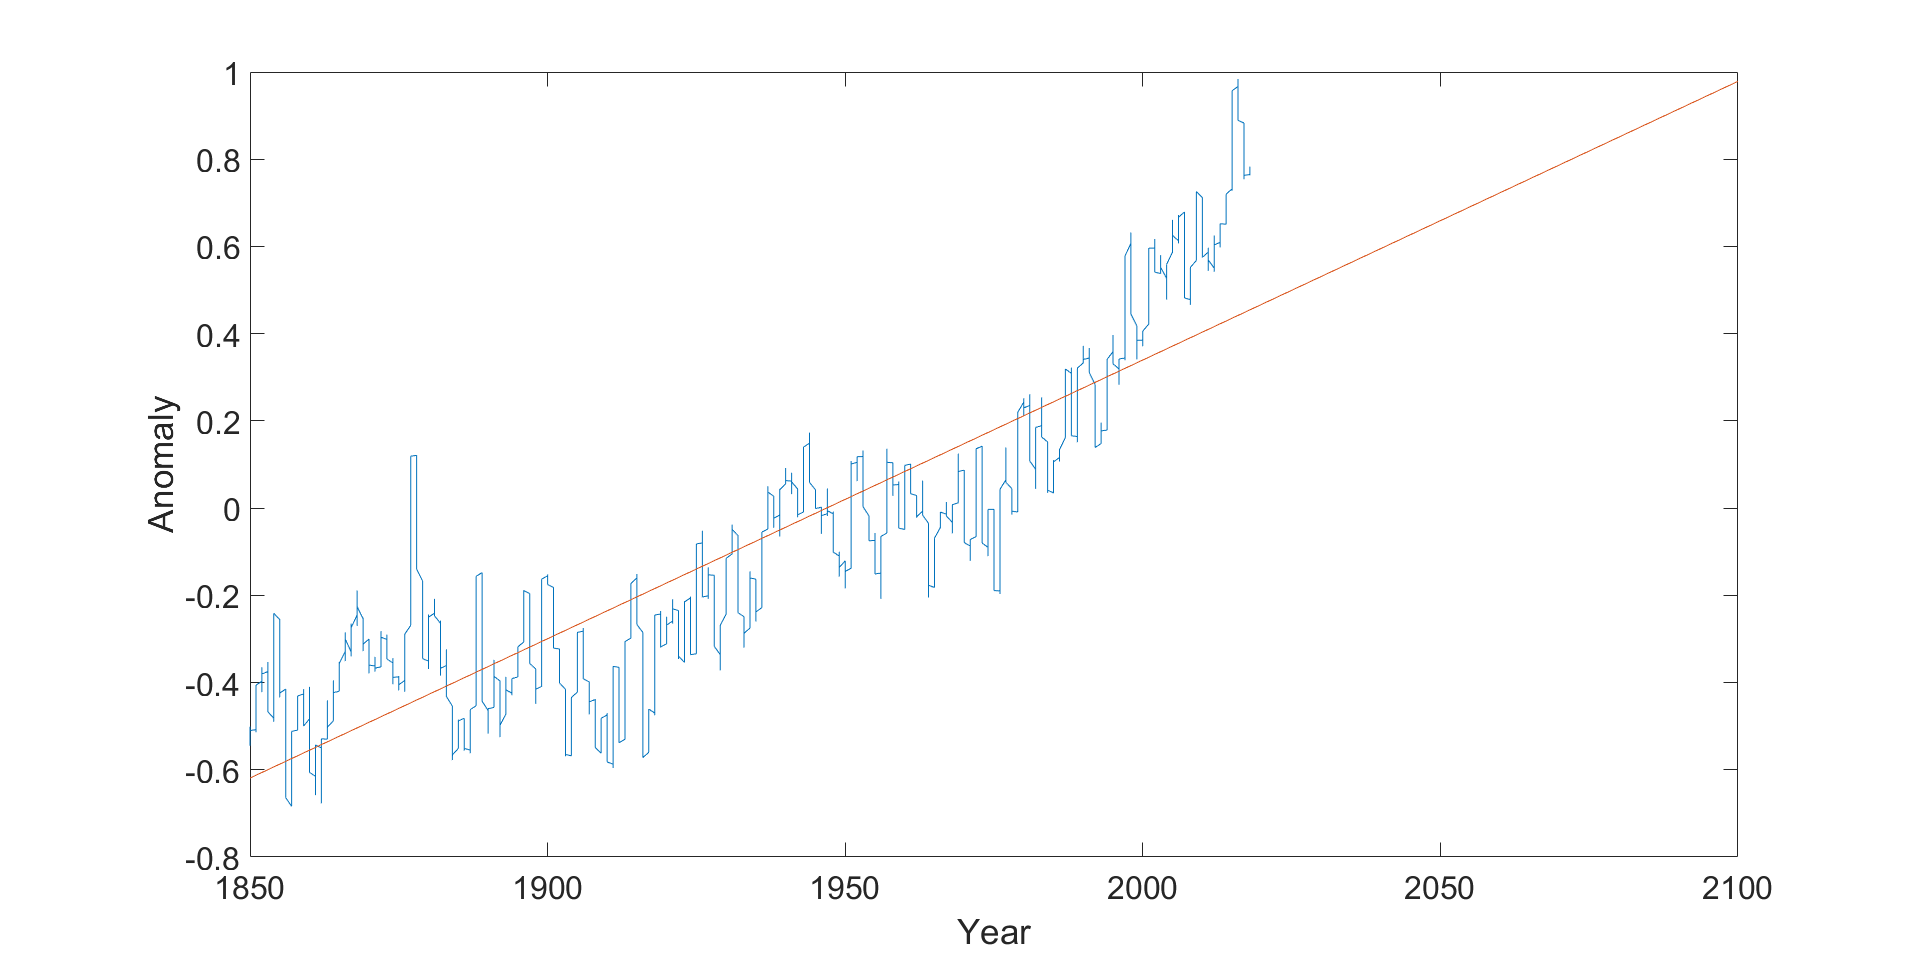
\includegraphics[width=\textwidth]{linear.png}
    \caption{Linear extrapolation of climate anomalies. The linear fit predicted an anomaly value of $9.79*10^{-1}$ in year 2100, with a cumulative error of $5.71*10^{1}$ calculated between the years 1850 and 2018.}
    \label{fig:linear}
\end{figure}

\begin{figure}[H]
    \centering
    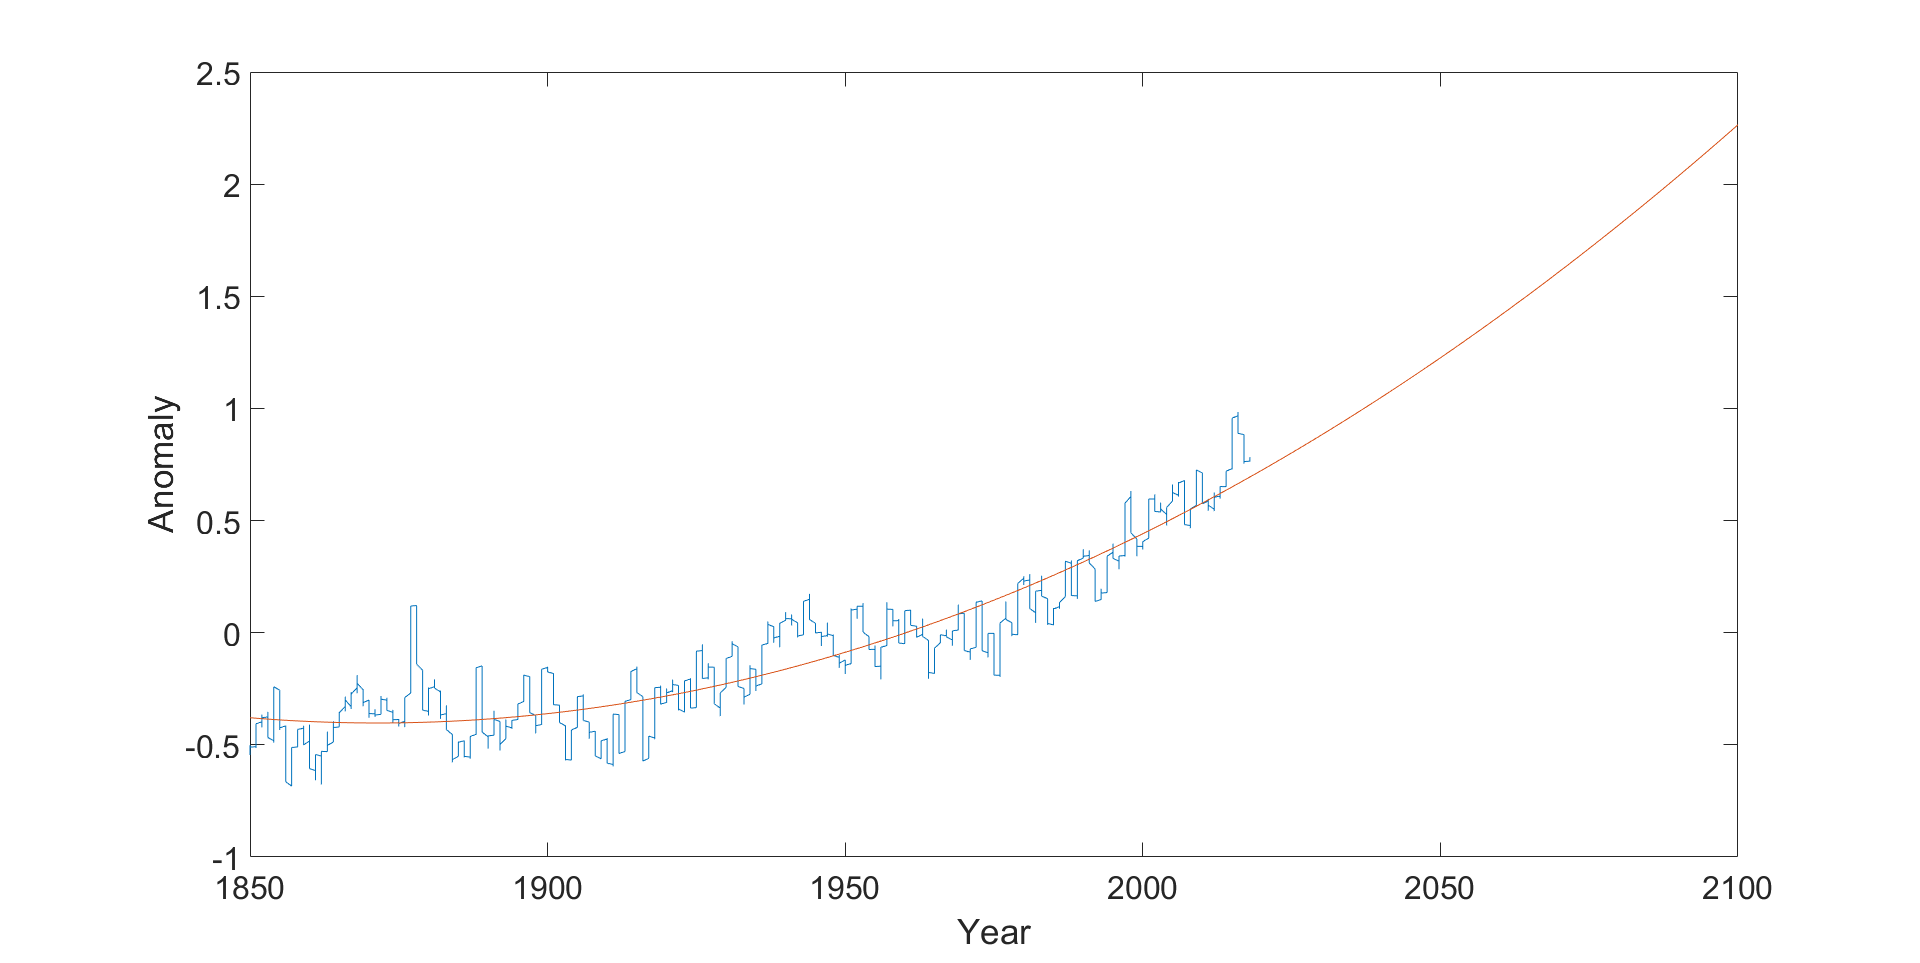
\includegraphics[width=\textwidth]{quadratic.png}
    \caption{Quadratic extrapolation of climate anomalies. The quadratic fit predicted an anomaly value of $2.26*10^{0}$ in year 2100, with a cumulative error of $3.38*10^{1}$ calculated between the years 1850 and 2018.}
    \label{fig:quadratic}
\end{figure}

\begin{figure}[H]
    \centering
    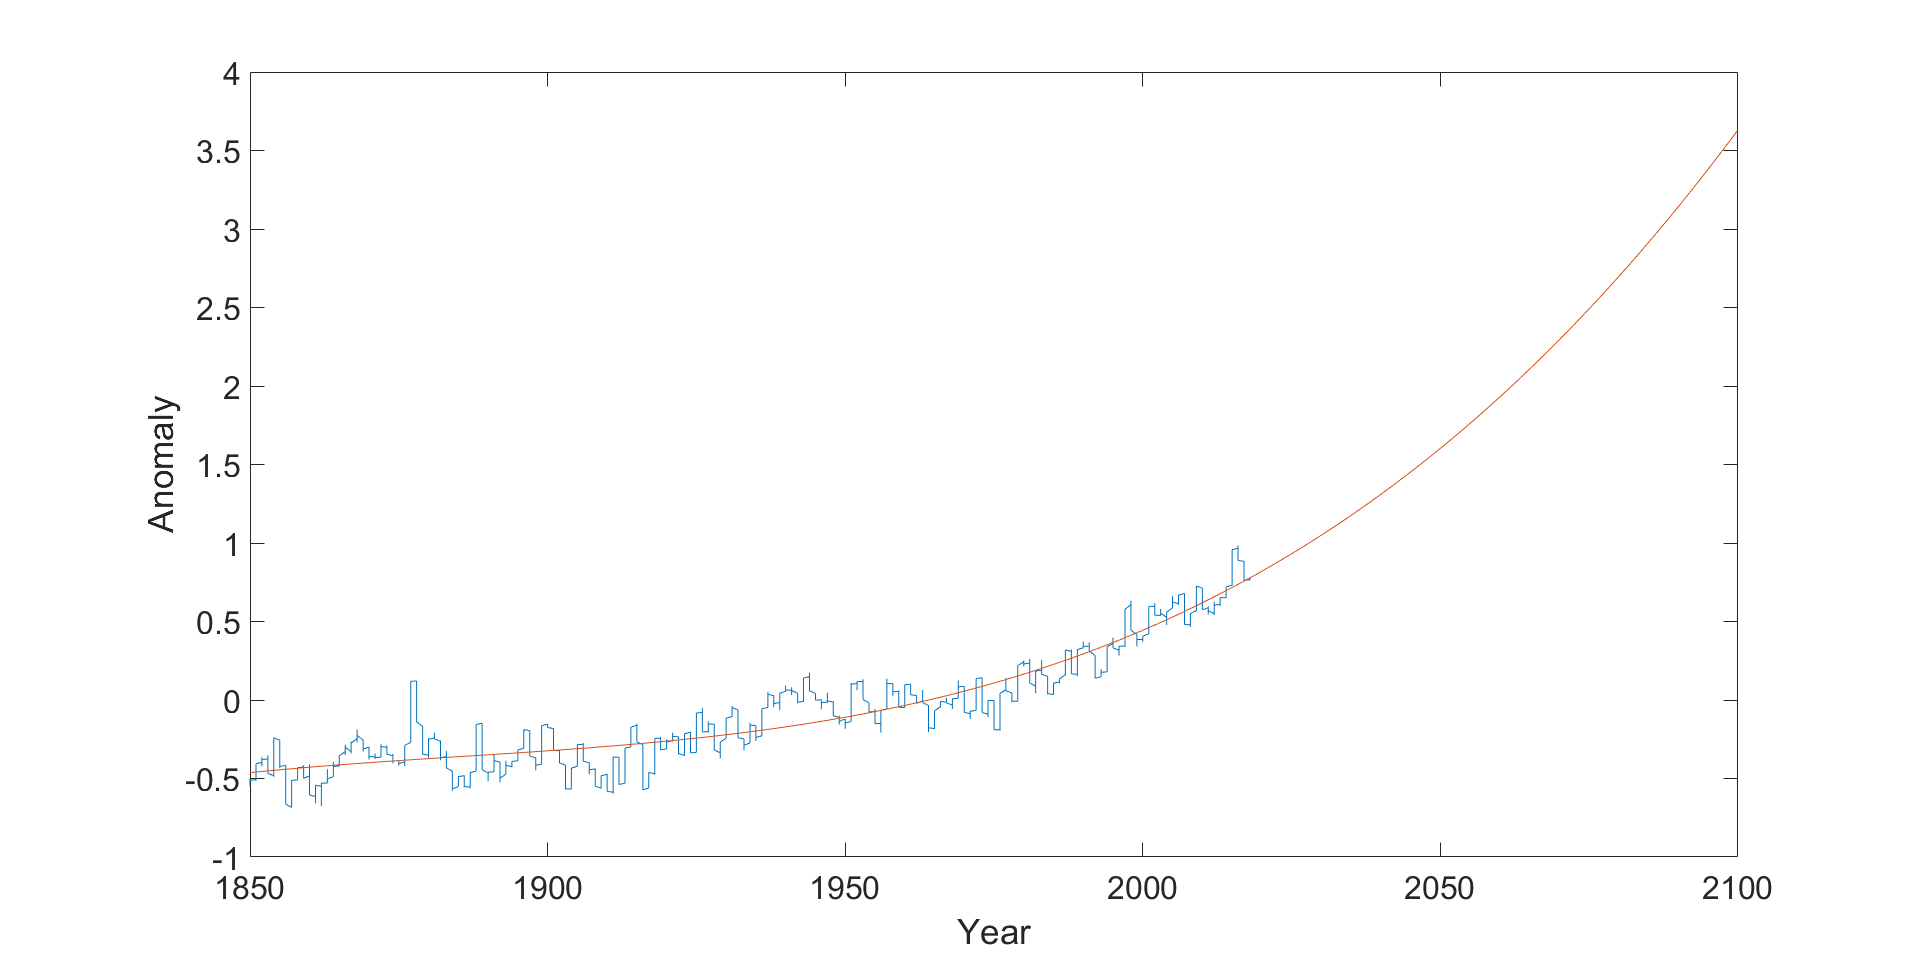
\includegraphics[width=\textwidth]{cubic.png}
    \caption{Cubic extrapolation of climate anomalies. The cubic fit predicted an anomaly value of $3.63*10^{0}$ in year 2100, with a cumulative error of $3.17*10^{1}$ calculated between the years 1850 and 2018.}
    \label{fig:cubic}
\end{figure}

\subsection{ Exponential and Mixed Fits}
After computing the data for an exponential fit, and two different mixed fits, the following results were obtained:

\begin{figure}[H]
    \centering
    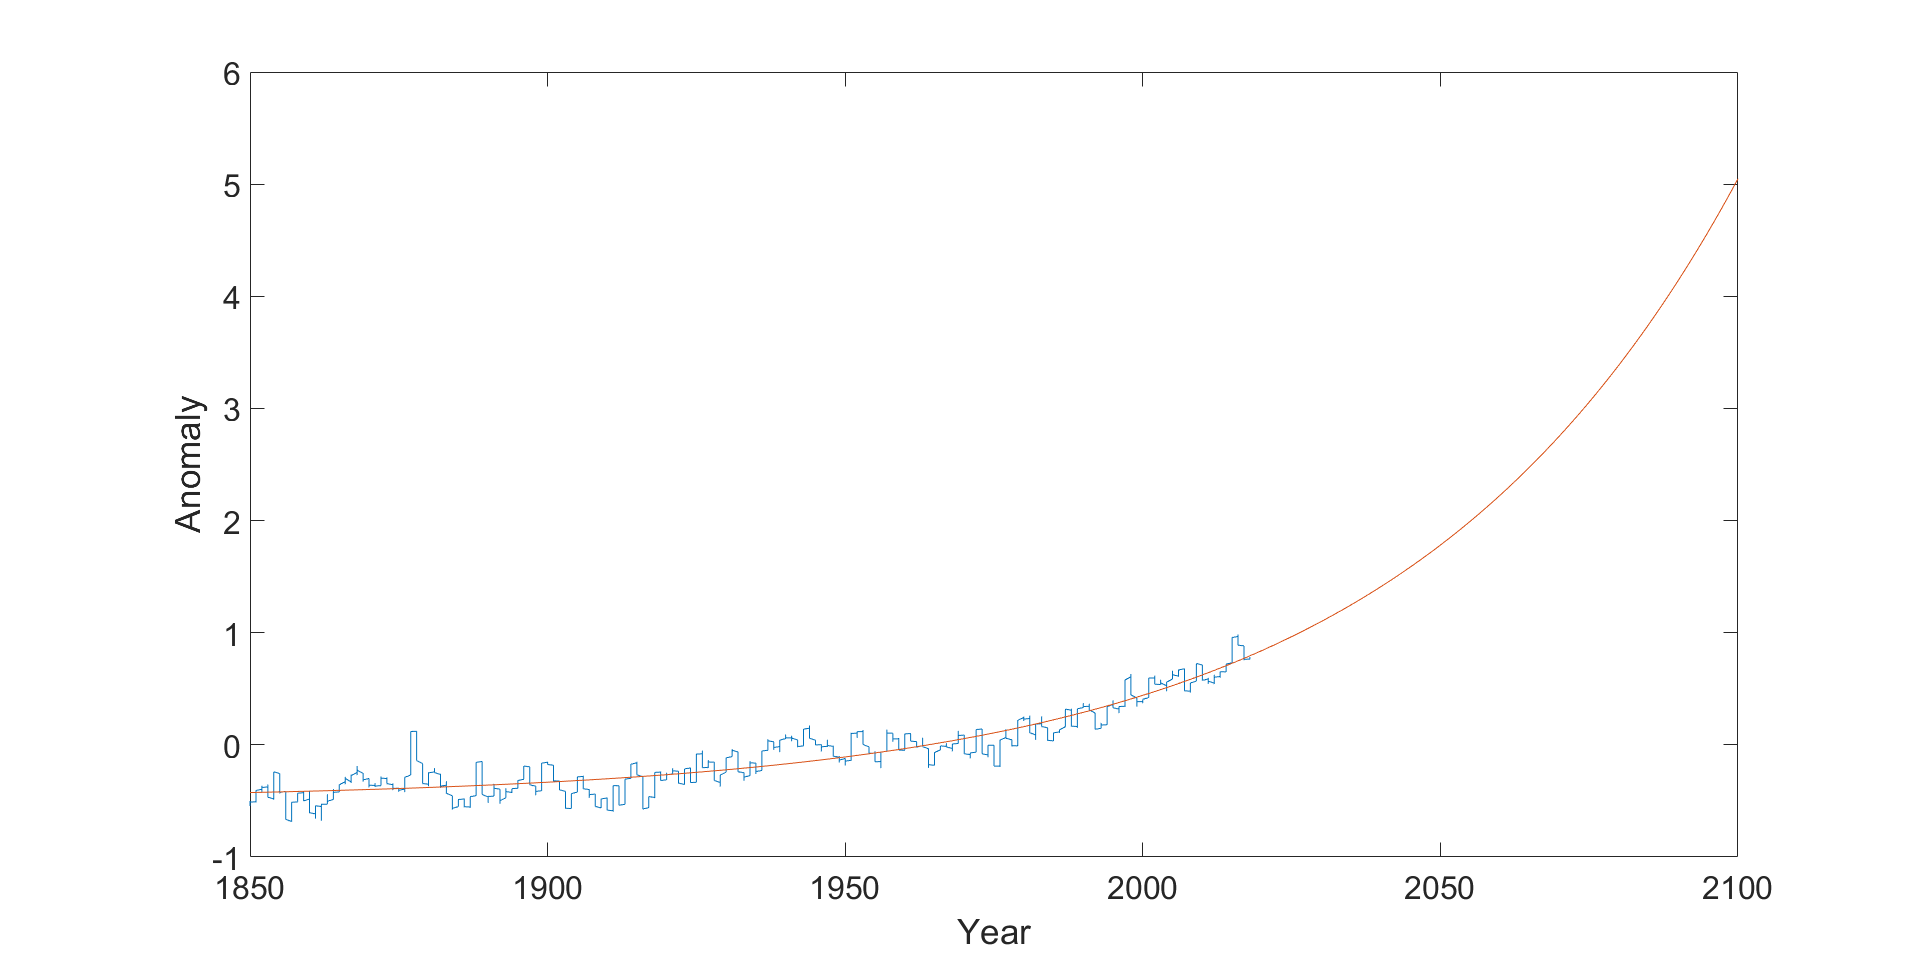
\includegraphics[width=\textwidth]{exp.png}
    \caption{Exponential extrapolation of climate anomalies. The exponential fit predicted an anomaly value of $5.04*10^0 $ in year 2100, with a cumulative error of $3.14*10^2 $ calculated between the years 1850 and 2018.}
    \label{fig:exp}
\end{figure}

\begin{figure}[H]
    \centering
    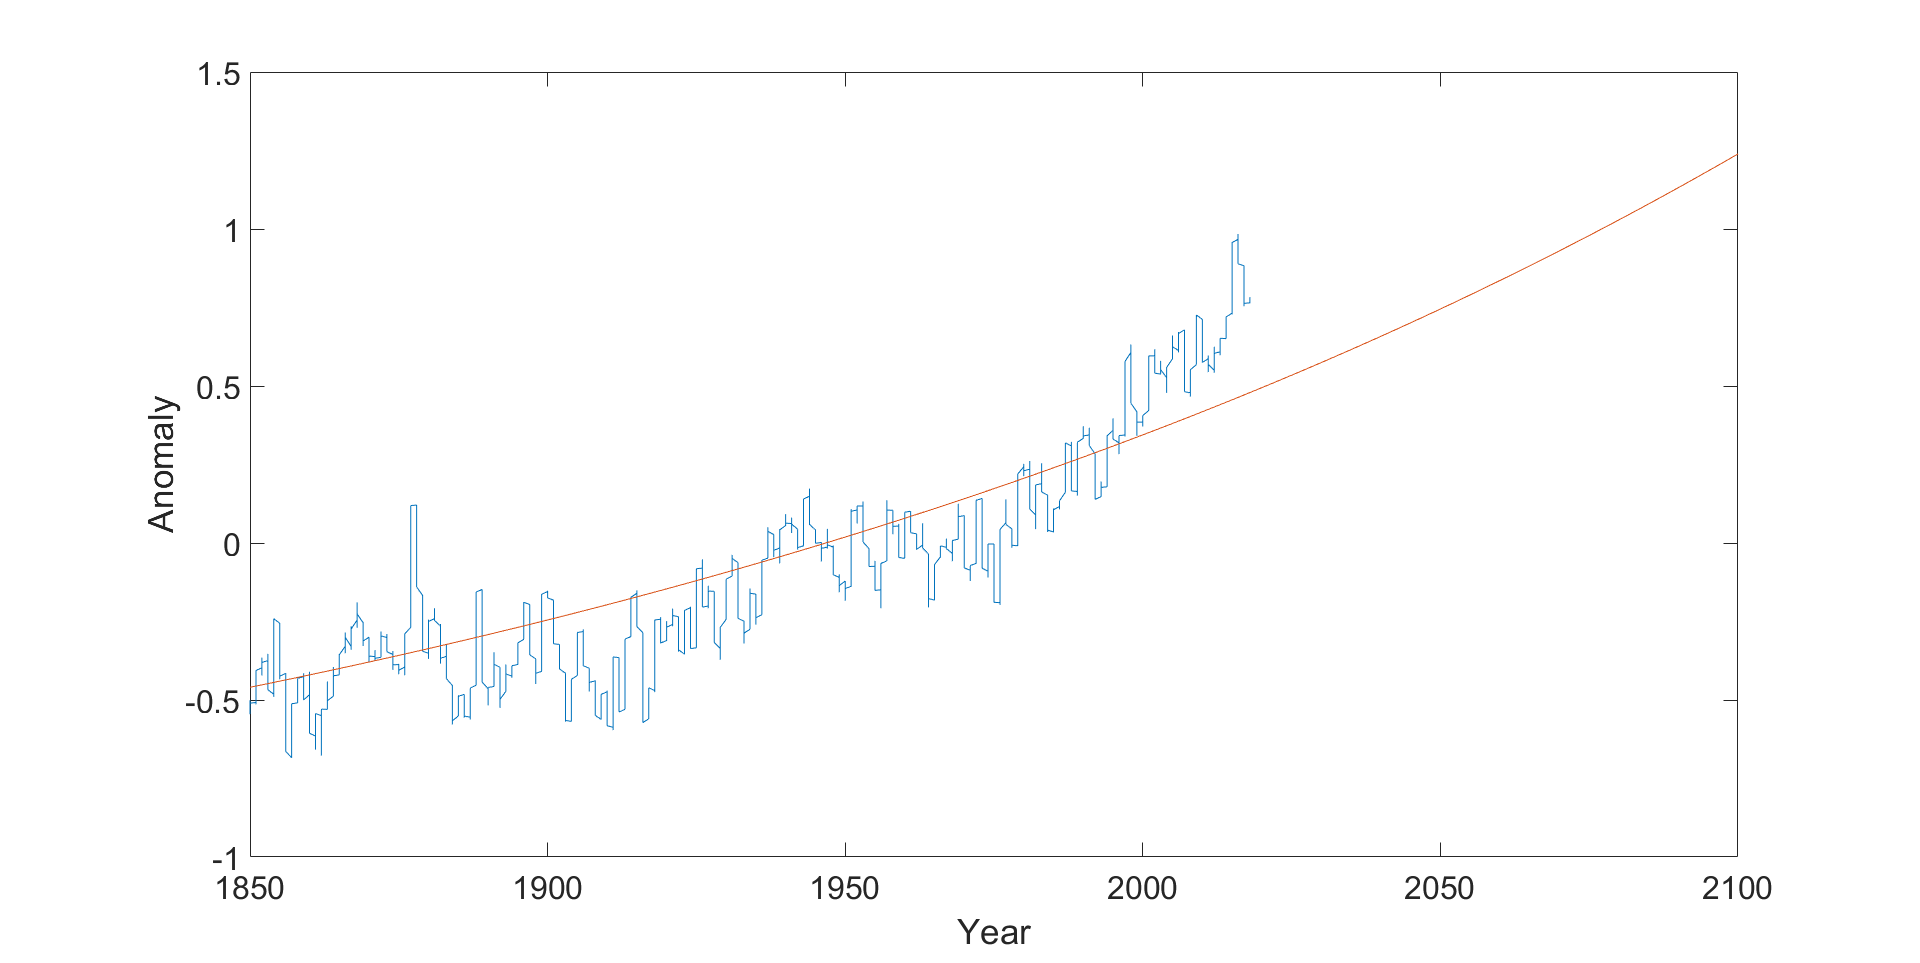
\includegraphics[width=\textwidth]{mix1.png}
    \caption{ Mixed exponential and linear extrapolation of climate anomalies. The mixed fit predicted an anomaly value of $ 1.32*10^0$ in year 2100, with a cumulative error of $4.89*10^1 $ calculated between the years 1850 and 2018.}
    \label{fig:mix1}
\end{figure}

\begin{figure}[H]
    \centering
    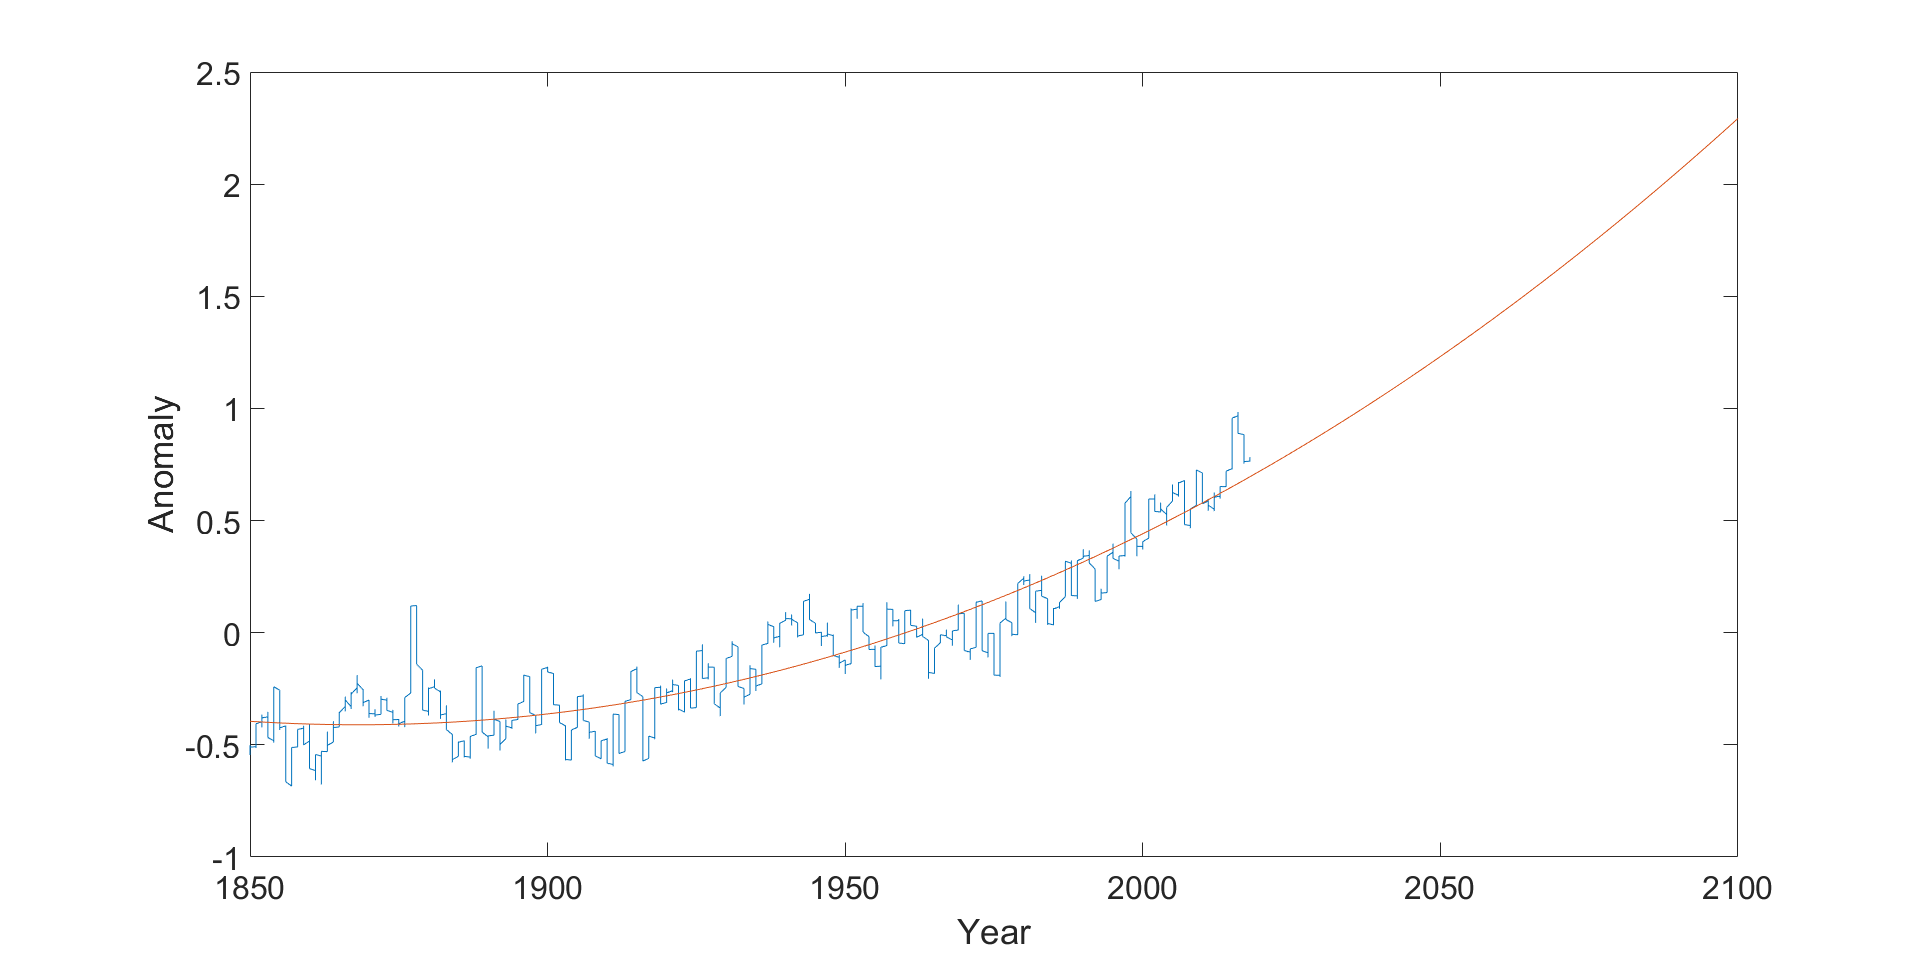
\includegraphics[width=\textwidth]{mix2.png}
    \caption{Mixed exponential and quadratic extrapolation of climate anomalies. The mixed fit predicted an anomaly value of $ 2.29*10^0$ in year 2100, with a cumulative error of $ 3.37*10^1$ calculated between the years 1850 and 2018.}
    \label{fig:mix2}
\end{figure}

\section{Analysis}
\subsection{Accuracy of Fit}
We can see that the fit becomes progressively more accurate as the degree of the polynomial increases, for both the mixed and purely polynomial fits. Initially, equation \eqref{eq:mix2} returned a nonsensical plot since it predicted a sharp decline in anomalies just past the last data point, but increasing the maximum iterations for \textit{lsqcurve}, we obtained a much more precise and logical fit. The interesting analysis we can make is that although equations \eqref{eq:mix1} and \eqref{eq:mix2} should have \textit{at least} the same amount of accuracy as \eqref{eq:exp} since we can simply set the coefficients of the polynomial portion to zero, it turns out due to computational limits that more error is introduced than eliminated. Matlab itself limits the number of computations allowed before it detects that the minimum difference of results between iterations has been reached and stops computing. Although the mixed results offer better fits than their purely polynomial counter parts, the cubic and exponential fits offer the most accurate fits according to the sum of the differences between the data points and the equation.\\
The fit with the lowest error appears to be the exponential fit, followed by the cubic fit. It is therefore likely that these two will offer the most accurate interpretation of the data.
\subsection{Interpretation of Results}
Both the exponential and cubic fit predict a far more aggressive increase in the anomaly value than any other fit, which is concerning. The exponential fit predicts an anomaly of $+31.4$ in the year 2100, while the cubic fit predicts an anomaly of $+31.7$. Considering the value has remained around 0.5 to 1 in 2018, for climate anomalies to triple or even quintiple is surely not a good sign. What this value means essentially is that we should expect to see more aggressive, unpredictible weather changes in the future if our impact on the environment does not change. Tornadoes, lightning storms, flash floods, and summer-time blizzards will become more and more common, which will impose a much higher cost in infrastructure maintenance and repair, and drastically increase the rate of injuries and deaths caused by weather.

\section{Conclusion and Future Considerations}
This project has helped demonstrate the utility of numerical analysis for predicting trends in areas such as climate, and also prompts the reader to consider the impact that our society has on the climate of our planet. For future improvements, one would potentially include more than just data from a single source, and improve the fit in areas such as extending computation time, using data types which can hold more precision for calculations, and using different equations altogether, such as a sin wave, as it appears from the graphs that there tends to be a trend where the anomaly value fluctuates in the shape of a wave. Reflecting on the trends at the time, such as vehicle and factory efficiency, and general consumerism would also help to improve accuracy, as those two areas are huge contributors to climate change.
\end{document}


